\documentclass{article}
\usepackage[utf8]{inputenc}
\usepackage{kotex}
\usepackage{amsmath}
\usepackage{graphicx}
\usepackage{subfigure}
\usepackage{verbatim}

\title{2022 Data Structure HW5}
\author{TaeYong Kim, C011060}
\date{\today}

\begin{document}

\maketitle

\section{Stack}
스택(stack)이란, 순서 리스트의 일종이다. 스택은 탑(top)이라고 하는 끝에서 모든 삽입(push)과 삭제(pop)이 일어난다. 스택의 특징은, 가장 마지막으로 삽입된 원소가 제일 먼저 삭제된다. 그래서 스택을 후입선출 (Last-In-First-Out, LIFO) 리스트라고 부른다.

\section{Homework}

\subsection{main}

\begin{verbatim}
int main()
{
  char line[MAXLEN];
  while (cin.getline(line, MAXLEN))
  {
    Expression e(line); // line 버퍼를 이용하여 Expression을 읽음
    try
    {
      // cout << "C011060\n";
      Postfix(e);
    }
    catch (char const *msg)
    {
      cerr << "Exception: " << msg << endl;
    }
  }
  return 0;
}
\end{verbatim}

\noindent \textbf{설명} \\
4행 while 조건문에 cin.getline() 함수를 통해 입력 값을 받는다. 


\subsection{GetInt}

\begin{verbatim}
bool GetInt(Expression &e, Token &tok)
{
  char arr[MAXLEN];
  int intlen = 0;
  char c = e.str[e.pos];
  if (!(c >= '0' && c <= '9'))
    return false;
  arr[intlen++] = c;
  e.pos++;
  while ((c = e.str[e.pos]) >= '0' && c <= '9')
  {
    arr[intlen++] = c;
    e.pos++;
  }
  arr[intlen] = '\0';
  tok = Token(arr, intlen, ID); // return an ID
  return true;
}
\end{verbatim}

\noindent \textbf{설명} \\
GetInt 함수는 전반적으로 GetID 함수와 비슷한 로직이다.
하지만, 6행과 10행의 조건문이 다르다.
GetInt 함수는 e.str[e.pos]가 정수형인지 아닌지를 판별해야 한다.
따라서, 6행에는 정수가 아닌 것들이면 false 반환하고, 10행에는 정수인 것들이면 arr[intlen]에 할당한 후, intlen을 1 증가 시킨다.

\subsection{TwoCharOp}

\begin{verbatim}
bool TwoCharOp(Expression &e, Token &tok)
{
  // 7가지 두글자 토큰들 <= >= == != && || -u을 처리
  char c1 = e.str[e.pos];
  char c2 = e.str[e.pos + 1];
  int op; // LE GE EQ NE AND OR UMINUS
  if (c1 == '<' && c2 == '=')
    op = LE;
  else if (c1 == '>' && c2 == '=')
    op = GE;
  else if (c1 == '=' && c2 == '=')
    op = EQ;
  else if (c1 == '!' && c2 == '=')
    op = NE;
  else if (c1 == '&' && c2 == '&')
    op = AND;
  else if (c1 == '|' && c2 == '|')
    op = OR;
  else if (c1 == '-' && c2 == 'u')
    op = UMINUS;
  else
  {
    return false;
  } // 맞는 두 글자 토큰이 아니면 false를 return
  tok = Token(c1, c2, op);
  e.pos += 2;
  return true;
}
\end{verbatim}

\noindent \textbf{설명} \\
TwoCharOp 함수는 7가지 두 글자 연산자를 처리하는 함수이다.
e.str[e.pos]와 e.str[e.pos + 1]을 각각 어떤 글자인지 확인하고, 해당 연산자를 반환한다.
if-else문으로 경우의 수를 모두 작성하여 구현했다.
그리고 e.pos는 2를 더해주어서 그 다음 글자를 확인할 수 있게 해준다.

\subsection{icp, isp}

\begin{verbatim}
int icp(Token &t)
{ // in-coming priority
  int ty = t.type;

  if (ty == '(')
    return 0;
  else if (ty == '!' || ty == UMINUS)
    return 1;
  else if (ty == '*' || ty == '/' || ty == '%')
    return 2;
  else if (ty == '+' || ty == '-')
    return 3;
  else if (ty == '<' || ty == '>' || ty == LE || ty == GE)
    return 4;
  else if (ty == EQ || ty == NE)
    return 5;
  else if (ty == AND)
    return 6;
  else if (ty == OR)
    return 7;
  else if (ty == '=')
    return 8;
  else if (ty == '#')
    return 10;
}

int isp(Token &t) // in-stack priority
{
  int ty = t.type; // stack 에서의 우선순위 결정
  // 이 부분 작성
  if (ty == '(')
    return 9;
  else
    return icp(t);
}
\end{verbatim}
\noindent \textbf{설명} \\
후위연산은 연산자의 우선순위를 반환하는 함수 두 가지가 필요하다. 하나는 isp(in-stack priority)와 icp(in-coming priorty)이다. 
\\
icp와 isp의 우선순위는 대부분 같다. 하지만, 다른 점은 isp는 '('를 8번째 우선순위를 반환하고, icp는 '('를 0번째 그리고 '#'을 8번째의 우선순위를 반환한다.
이러한 우선순위에 따라 다음의 규칙이 성립된다.
\\
연산자는 자신의 isp가 새로운 연산자의 icp보다 작거나 같을 때, 스택 밖으로 나온다.


\subsection{Postfix}

\begin{verbatim}
void Postfix(Expression e)
{
  stack<Token> stack;
  stack.push('#');

  for (Token x = NextToken(e); x != '#'; x = NextToken(e))
  {
    if (x.IsOperand())
    {
      cout << x;
    }
    else if (x == ')')
    {
      for (; stack.top() != '('; stack.pop())
      {
        cout << stack.top();
      }
      stack.pop();
    }
    else
    {
      for (; isp(stack.top()) <= icp(x); stack.pop())
      {
        cout << stack.top();
      }
      stack.push(x);
    }
  }
  while (stack.top() != '#')
  {
    cout << stack.top();
    stack.pop();
  }
  stack.pop();

  cout << endl;
}
\end{verbatim}

\noindent \textbf{설명} \\
Postfix 함수는 후위연산을 하는 함수이다. 먼저, stack이라는 스택을 초기화하고, '\#'을 삽입한다. '\#'는 스택의 밑 부분이라는 것을 표시한다. 그리고 for문을 통해 e를 토큰 단위로 받고, 이를 끝까지 즉, '\#'이 나올 때까지 반복한다. 만약 토큰 x가 연산자라면 출력하고, ')'이라면 '('이 나올때까지 스택을 출력하고 삭제한다. 그리고 이에 해당하지 않으면, 즉 x가 연산자라면 우선순위를 계산해 연산자가 자신의 isp가 새로운 연산자의 icp보다 작거나 같을 때 x를 출력하고 삭제한다.




\section{Conclusion}
Postfix의 알고리즘 분석을 해보자. 입력되는 값들은 왼쪽에서 오른쪽으로 입력된다. 각 피연산자에 소요되는 시간은 O(1)이다. 각 연산자들은 한 번씩만 스택에 삽입과 삭제가 된다. 그러므로, 각 연산자에 소요되는 시간 또한 O(1)이 된다. 따라서, 토큰의 수가 n이라고 가정할 때, Postfix 함수의 시간 복잡도는 O(n)이 된다.
\\
마지막으로, 다음은 본 코드를 실행하고 테스트를 했을 때의 결과이다.
\\
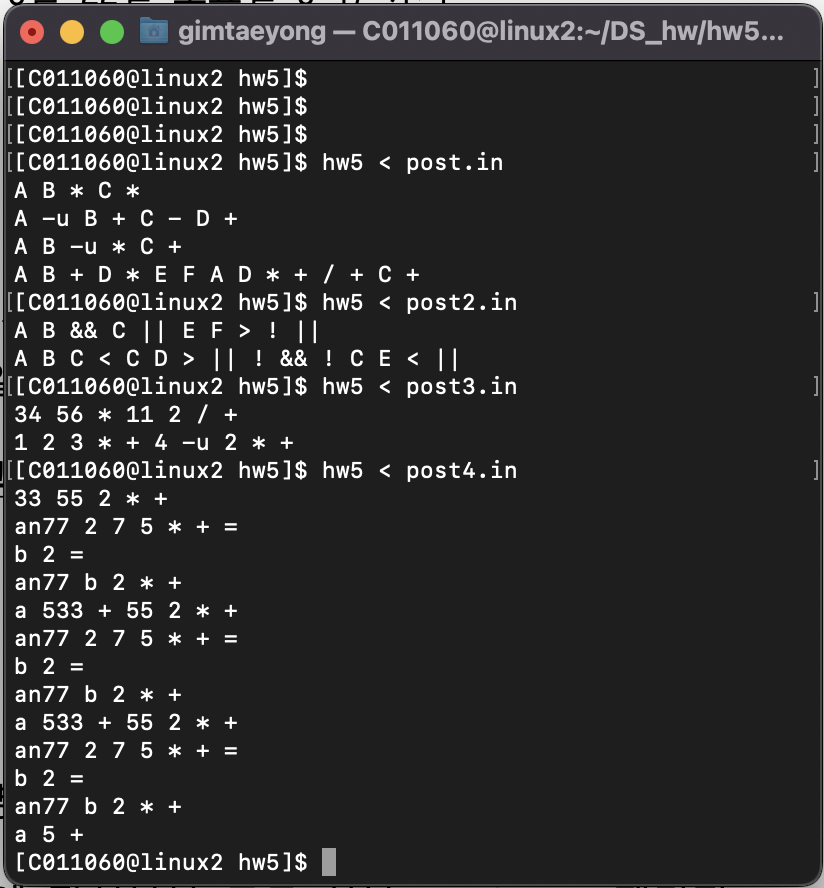
\includegraphics{result.png}
\\
끝.
\end{document}
